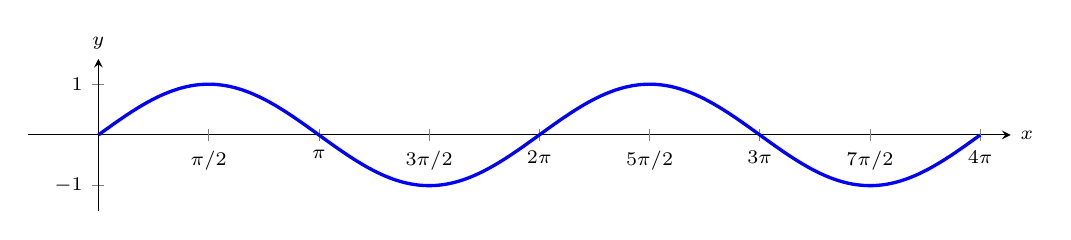
\begin{tikzpicture}
\begin{axis}[width=400pt,height=100pt,%
tick label style={font=\scriptsize},axis y line=middle,axis x line=middle,name=myplot,%
			%x=.37\marginparwidth,
			%y=.37\marginparwidth,
			xtick=\empty,% 
			extra x ticks={1.5708, 3.14159, 4.71239, 6.28319, 7.85398, 9.42478, 10.9956, 12.5664},
			extra x tick labels={$\pi/2$,$\pi$,$3\pi/2$,$2\pi$,$5\pi/2$,$3\pi$,$7\pi/2$,$4\pi$},
			ytick={-1,1},
			%minor y tick num=1,%extra y ticks={-5,-3,...,7},%
			ymin=-1.5,ymax=1.5,%
			xmin=-1,xmax=13%
]

\addplot [very thick,blue,smooth,domain=0:12.566,samples=100] {sin(deg(x))};
%\draw [dashed,thick] (axis cs:-3,-37) -- (axis cs:3,47);
%\filldraw (axis cs:-3,-37) circle (1pt);
%\filldraw (axis cs:3,47) circle (1pt);
%\filldraw (axis cs:-1.732,-8.86) circle (.75pt);
%\addplot [thick,dashed,domain=-2.8:-.1,{\colortwo}] {14*(x+1.732)-13.86+5};
%\filldraw (axis cs:1.732,18.86) circle (.75pt);
%\addplot [thick,dashed,domain=-.1:3,{\colortwo}] {14*(x-1.732)+13.86+5};
\end{axis}

\node [right] at (myplot.right of origin) {\scriptsize $x$};
\node [above] at (myplot.above origin) {\scriptsize $y$};
\end{tikzpicture}
